%% Layout of a paper figure, filled by scripts/exporters/export_paper_figs.py: every %%PLOTS%% line is replaced by the
%% plots of one axis, in order. Lines starting with %% are dropped from the output.
% Zero-shot classification controls of Qwen3-32B (appendix).
% Requires pgfplots (compat=1.18), xcolor and graphicx.
\begin{figure}[ht]
\centering
\def\plotwidth{3.5cm}
\mbox{\tikz[baseline=-0.6ex]\draw[brown!70!black, dashed, line width=0.8pt] plot coordinates {(0,0) (0.4,0)}; {\small Foo/Bar}}\hspace{1em}%
\mbox{\tikz[baseline=-0.6ex]\draw[blue!60!black, dashed, line width=0.8pt] plot coordinates {(0,0) (0.4,0)}; {\small Rotation/Permutation}}\hspace{1em}%
\mbox{\tikz[baseline=-0.6ex]\draw[green!70!black, dashed, line width=0.8pt] plot coordinates {(0,0) (0.4,0)}; {\small Vanilla/Chocolate}}\hspace{1em}%
\mbox{\tikz[baseline=-0.6ex]\draw[cyan!40!blue!70, dashed, line width=0.8pt] plot coordinates {(0,0) (0.4,0)}; {\small X/Y}}\\[2pt]
\resizebox{0.6\linewidth}{!}{%
\begin{minipage}{\plotwidth}
  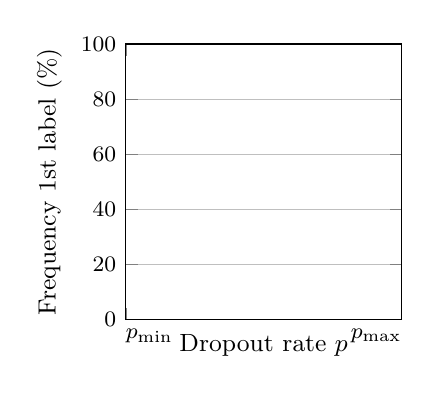
\begin{tikzpicture}
\begin{axis}[
    height=\plotwidth,
    width=\plotwidth,
    scale only axis,
    grid=major,
    xlabel={\small Dropout rate $p$},
    ylabel={\small Frequency 1st label (\%)},
    xmin=0, xmax=100,
    xtick={0,100},
    xticklabels={\makebox[0pt][l]{$p_{\min}$},\makebox[0pt][r]{$p_{\max}$}},
    ymin=0.0, ymax=100.0,
    ytick={0,20,40,60,80,100},
    tick label style={font=\footnotesize},
    xlabel style={yshift=1em},
]
%%PLOTS%%
\end{axis}
\end{tikzpicture}
\end{minipage}%
\hspace{1.5cm}%
\begin{minipage}{\plotwidth}
  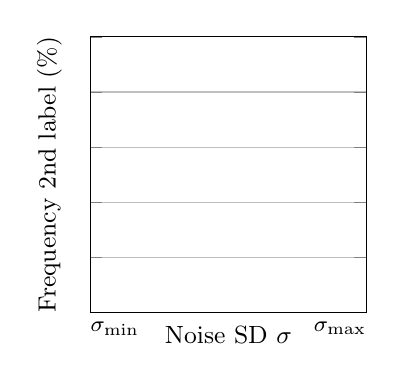
\begin{tikzpicture}
\begin{axis}[
    height=\plotwidth,
    width=\plotwidth,
    scale only axis,
    grid=major,
    xlabel={\small Noise SD $\sigma$},
    ylabel={\small Frequency 2nd label (\%)},
    yticklabels={},
    xmin=0, xmax=100,
    xtick={0,100},
    xticklabels={\makebox[0pt][l]{$\sigma_{\min}$},\makebox[0pt][r]{$\sigma_{\max}$}},
    ymin=0.0, ymax=100.0,
    ytick={0,20,40,60,80,100},
    tick label style={font=\footnotesize},
    xlabel style={yshift=1em},
]
%%PLOTS%%
\end{axis}
\end{tikzpicture}
\end{minipage}%
}
\caption{\small
Zero-shot classification controls of \model{qwen32}. We alias the concepts, asking \eg, \emph{``Did we apply X or Y?''} while still applying either dropout (left) or noise (right), and report the \textbf{frequency} of times the model answers, \eg, ``X'' (resp.\ ``Y'') when dropout (resp.\ noise) is applied (frequency under the correct labels coincides with accuracy).
}
\label{fig:zero_shot_controls}
\end{figure}
